\section{Wednesday for MAT4002}\index{Monday_lecture}
\subsection{Remarks on Triangulation}
Consider the simplical complex $K=(V,\Sigma)$ with
\[
V=\{1,2,3,4,\dots,9\},\quad
\Sigma=\left\{
\begin{aligned}
\text{$9$ subsets with $1$ element}\\
\text{$27$ subsets with $2$ elements}\\
\text{$18$ subsets with $3$ elements}
\end{aligned}
\right.
\]
We start to build the topological realization of $K$ with $9$ $\bm0$-simplicies, $27$ $\bm1$-simplicies, and $18$ $\bm2$-simplicies. The identification of them is as follows:
\begin{figure}[H]
\centering
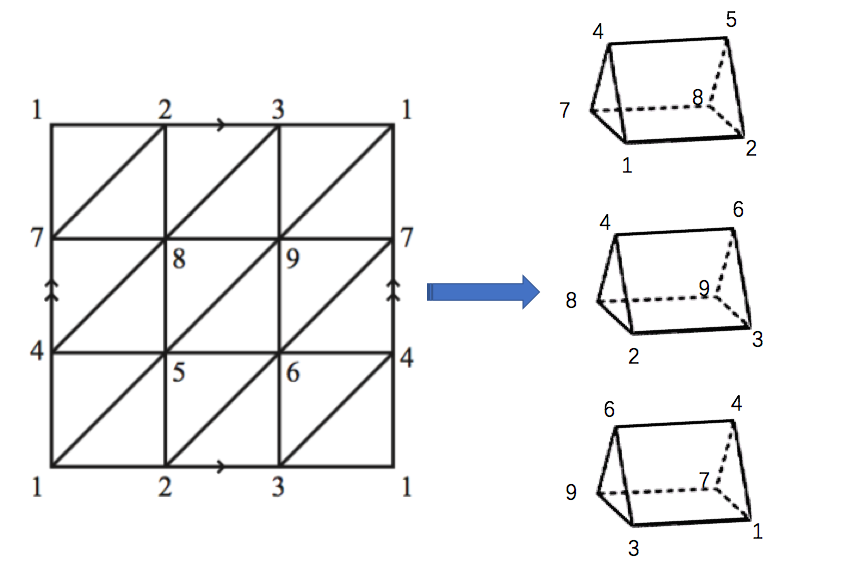
\includegraphics[width=0.5\textwidth]{week7/p_10}
\caption{Step 1: Identify 3 columns separately, i.e., identify $\{1,7,4,1,2,8,5,2\}$, $\{2,8,5,2,3,9,6,3\}$, and $\{3,9,6,3,1,7,4,1\}$.}
\end{figure}
\begin{figure}[H]
\centering
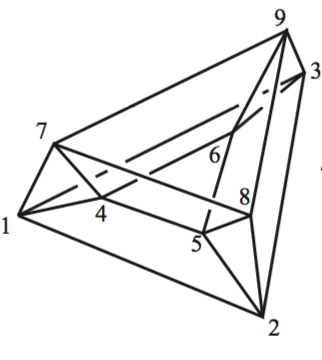
\includegraphics[width=0.3\textwidth]{week7/p_11}
\caption{Step 2: ``gluing'' these three prisms in the figure above together.}
\end{figure}

Question: why $K$ is homeomorphic to the torus?

\begin{example}
Consider the simplicial complex $(V,\Sigma)$ described below:
\begin{figure}[H]
\centering
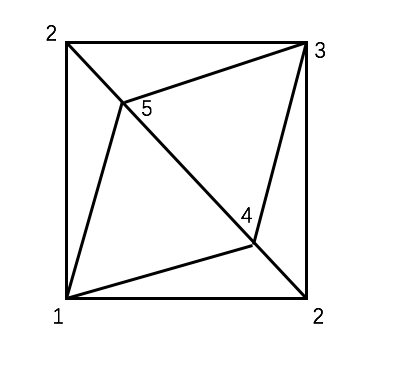
\includegraphics[width=0.4\textwidth]{week7/p_12}
\end{figure}
The $|(V,\Sigma)|$ is homeomorphism to the quotient space $S^1$ plotted below
\begin{figure}[H]
\centering
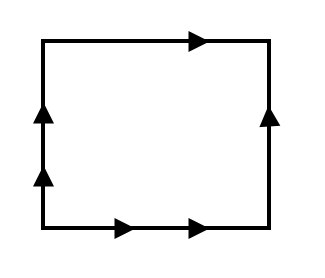
\includegraphics[width=0.3\textwidth]{week7/p_13}
\end{figure}
\end{example}





Furthermore, can we build a triangulation of the tours using fewer simplices? The answer is no.
Consider the figure below: at the bottom edge of this square, there are two 1-simplicies lablled $\{1,2\}$, which cannot happen in a tours.
\begin{figure}[H]
\centering
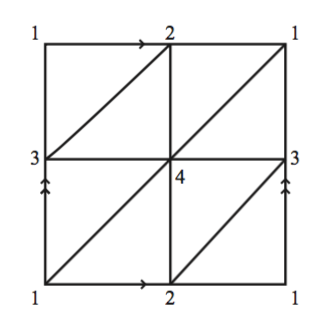
\includegraphics[width=0.4\textwidth]{week7/p_14}
\end{figure}

Interesting question: does the triangulation of the Fig.~(7.1a) below leads to $S^2$? 
\begin{figure}[H]
\centering
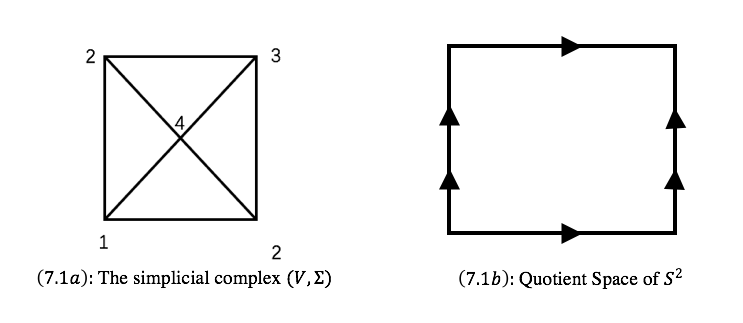
\includegraphics[width=0.9\textwidth]{week7/p_15}
\end{figure}
Answer: No.
Since the 2-simplex $\Delta_{\{2,3,4\}}$ appears twice in the Fig.~(7.1a), the triangluation of this figure means that we need to stick the top triangle and the right triangle together, which contradicts to the structure of the quotient space $S^2$ shown in Fig.~(7.1b).


The simplicial complex gives us another way to study $X$, i.e., it suffices to study $(V,\Sigma)$ such that $|(V,\Sigma)|\cong X$.
The question is that can we distinguish $X=S^1\times S^1$ and $Y=S^2$?
In other words, can we distinguish the difference of corresponding topological realizations? 

\begin{theorem}[Euler's Formula]
Suppose that $|(V_1,\Sigma_1)|\cong|(V_2,\Sigma_2)|$, then 
\begin{align*}
&\sum_{i=1}^\infty(-1)^i\left(\text{number of subsets in $\Sigma_1$ with $(i+1)$-element}\right)\\
&=
\sum_{i=1}^\infty(-1)^i\left(\text{number of subsets in $\Sigma_2$ with $(i+1)$-element}\right)
\end{align*}
\end{theorem}

From previous examples we can see that $\mathcal{X}(S^2) = 5-9+6=2$ and $\mathcal{X}(S^1\times S^1) = 9-27+18=0$, which implies
\[
S^2\not\cong S^1\times S^1.
\]

\subsection{Simplicial Subcomplex}

\begin{definition}[Simplicial Subcomplex]
A subcomplex of a simplicial complex $K=(V,\Sigma)$ is a simplicial complex $K'=(V',\Sigma')$ such that 
\[
V'\subseteq V,\quad
\Sigma'\subseteq\Sigma
\]
\end{definition}
\begin{proposition}
Suppose $K'$ is subcomplex of $K$, then $|K'|$ is closed in $|K|$.
\end{proposition}
\begin{proof}
Suppose that $D$ is the disjoint union of all the simplicial complex forming $|K|$. (note that the number of component in $D$ is $|\Sigma|$)

Consider the canonical projection mapping $D\to|K|$. Observe that $p^{-1}(|K'|)$ precisely equals to $\coprod_{\sigma'\in\Sigma'}\sigma'$, which is closed in $D$.
By definition of quotient topology, $|K'|$ is also closed. 
\end{proof}

\begin{definition}[Subcomplex spanned by vertices]
Let $K=(V,\Sigma)$ be a simplicial complex and $V'\subseteq V$.
Then the subcomplex spanned by $V'$ is $(V',\Sigma')$ such that
\begin{itemize}
\item
$V'$ denotes the vertex set.
\item
the simplices $\Sigma'$ is given by
\[
\{\sigma\in\Sigma\mid\sigma\subseteq V'\}
\]
\end{itemize}
\end{definition}

\begin{definition}[Link and Star]
Let $(V,\Sigma)=K$ be simplicial complex
\begin{itemize}
\item
The \emph{link} of $\bm v\in V$, denoted as $\text{lk}(\bm v)$ is the sub-complex with
\begin{itemize}
\item
vertex set
\[
\{\bm w\in V\setminus\{\bm v\}\mid \{\bm v,\bm w\}\in\Sigma\}
\]
\item
simplicies
\[
\{\sigma\in\Sigma\mid\bm v\notin\sigma\text{ and }\sigma\cup\{\bm v\}\in\Sigma\}
\]
\end{itemize}
\item
The star of $\bm v$~(denoted as $\text{st}(\bm v)$) is
\[
\bigcup\{\text{inside}(\sigma)\mid \sigma\in\Sigma,\bm v\in\sigma\}
\]
\end{itemize}
\end{definition}

\begin{proposition}
$\text{st}(\bm v)$ is open and $\bm v\in\text{st}(\bm v)$.
\end{proposition}
\begin{proof}
Omitted.
\end{proof}
In fact, $|K|\setminus\text{st}(\bm v)$ is the simplicial subcomplex spanned by $V$.

\subsection{Some properties of simplicial complex}

\begin{proposition}
Suppose that $K=(V,\Sigma)$, where $V$ is finite.
Then $|K|$ is compact.
\end{proposition}
\begin{proof}
The mapping $p:D\to|K|$ is a canonical projection mapping, which is continuous; and 
$D$ (the finite disjoint union of $\Delta_\sigma$'s) is compact.

Therefore, $p(D)=|K|$ is compact.
\end{proof}

\begin{proposition}
For any simplicial complex $K=(V,\Sigma)$, where $V$ is finite, there is a continuous injection
\[
f:|K|\to\mathbb{R}^n\ \text{ for some $n$}
\]
\end{proposition}
\begin{proof}
Let $K'=(V,\Sigma')$, where $\Sigma'=\text{power set of $V$}$. Then
\[
|K'| = \Delta^{|V|-1}\subseteq \mathbb{R}^{|V|}
\]
Consider the inclusion
\[
i:|K|\to|K'|
\]
which comes from the following:
\begin{enumerate}
\item
Consider the $D:=\coprod_{\sigma\in \Sigma}\Delta_{\sigma}$ and $D'=\coprod_{\sigma'\in \Sigma'}\Delta_{\sigma'}$ in $(V,\Sigma)$ and $(V,\Sigma')$
\item
Construct the mapping $\tilde{i}:D\hookrightarrow D'\xrightarrow{p'}|K|$.
\item
The mapping $\tilde{i}$ descends to $i:D/\sim\to|K'|$~(try to write down the detailed mapping), which is continuous and injective.
\end{enumerate}
Therefore, $|K|\hookrightarrow|K'|$, i.e., $|K|\hookrightarrow\mathbb{R}^n$.
The proof is complete.

\end{proof}














